\subsection{Постановка задачи}
Для указанной функции провести модульное тестирование разложения функции в степенной ряд. Выбрать достаточное тестовое покрытие.
\subsection{Функция}
Функция $ sin(x) $
\subsection{Исходный код}
\lstinputlisting[language=java]{../src/main/java/testing/lab1/Calculator.java}
\subsection{Тесты}
\lstinputlisting[language=java]{../src/test/java/testing/lab1/CalculatorTest.java}
\subsection{Обоснование тестового покрытия}
Первая группа тестов проверяет, что синус не выходит за пределы $ [-1; 1] $.
Эта группа дополняет следующую, которая демонстрирует, что в примечательных точках
наш синус даёт корректные результаты. На Рис. \ref{f:sin-cover} показано, как
выбраны данные точки.
\begin{figure}[H]
  \centering
  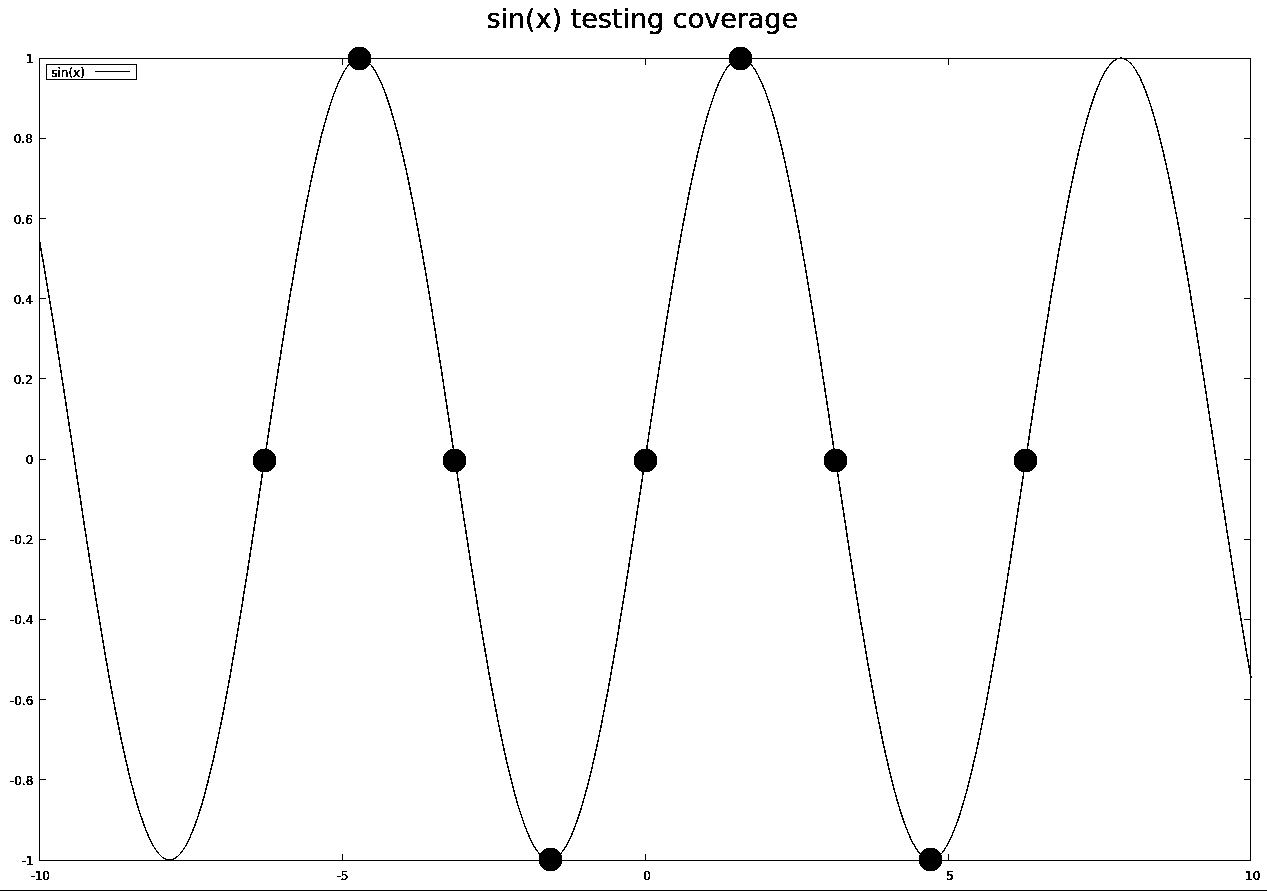
\includegraphics[scale=0.5]{./sin-cover.png}
  \caption{Тестовое покрытие для $ sin(x) $}
  \label{f:sin-cover}
\end{figure}

Таким образом, проверка периодичность появления примечательных точек ( $ -2\pi $,
$ -\frac{3}{2}\pi $, $ -\pi $, $ -\frac{1}{2}\pi $, $ 0 $, $ \frac{1}{2}\pi $,
$ \pi $, $ \frac{3}{2}\pi $, $ 2\pi $) и общее попадание в теоретическое множество
значений функции синуса в рамках, в которых применимо разложение в ряд Тейлора,
позволяет сделать положительный вывод о качестве реализованного алгоритма вычисления
синуса.
